\documentclass{article}
\usepackage[sc]{mathpazo}
\usepackage[T1]{fontenc}
\usepackage{geometry}
\geometry{verbose,tmargin=2.5cm,bmargin=2.5cm,lmargin=2.5cm,rmargin=2.5cm}
\setcounter{secnumdepth}{2}
\setcounter{tocdepth}{2}
\usepackage{url}
\usepackage[unicode=true,pdfusetitle,
 bookmarks=true,bookmarksnumbered=true,bookmarksopen=true,bookmarksopenlevel=2,
 breaklinks=false,pdfborder={0 0 1},backref=false,colorlinks=false]
 {hyperref}
\hypersetup{
 pdfstartview={XYZ null null 1}}
\usepackage{breakurl}
\begin{document}



\author{Ricky Lim}
\title{Lesson3}
\maketitle

\section{Prelude}
\begin{knitrout}
\definecolor{shadecolor}{rgb}{0.969, 0.969, 0.969}\color{fgcolor}\begin{kframe}
\begin{alltt}
\hlstd{work_dir} \hlkwb{=} \hlstr{'/Users/RickyLim/Documents/OnlineLearning/DataAnalysisR/'}
\hlkwd{library}\hlstd{(ggplot2)}
\end{alltt}
\end{kframe}
\end{knitrout}

\section{Dataset}
\begin{knitrout}
\definecolor{shadecolor}{rgb}{0.969, 0.969, 0.969}\color{fgcolor}\begin{kframe}
\begin{alltt}
\hlstd{pf} \hlkwb{<-} \hlkwd{read.csv}\hlstd{(}\hlkwd{paste0}\hlstd{(work_dir,} \hlstr{'Data/pseudo_facebook.tsv'}\hlstd{),}
               \hlkwc{sep} \hlstd{=} \hlstr{'\textbackslash{}t'}\hlstd{)}
\hlkwd{dim}\hlstd{(pf)}
\end{alltt}
\begin{verbatim}
## [1] 99003    15
\end{verbatim}
\begin{alltt}
\hlkwd{head}\hlstd{(pf)}
\end{alltt}
\begin{verbatim}
##    userid age dob_day dob_year dob_month gender tenure friend_count friendships_initiated
## 1 2094382  14      19     1999        11   male    266            0                     0
## 2 1192601  14       2     1999        11 female      6            0                     0
## 3 2083884  14      16     1999        11   male     13            0                     0
## 4 1203168  14      25     1999        12 female     93            0                     0
## 5 1733186  14       4     1999        12   male     82            0                     0
## 6 1524765  14       1     1999        12   male     15            0                     0
##   likes likes_received mobile_likes mobile_likes_received www_likes www_likes_received
## 1     0              0            0                     0         0                  0
## 2     0              0            0                     0         0                  0
## 3     0              0            0                     0         0                  0
## 4     0              0            0                     0         0                  0
## 5     0              0            0                     0         0                  0
## 6     0              0            0                     0         0                  0
\end{verbatim}
\end{kframe}
\end{knitrout}

\subsection{User's Birthday}
\begin{knitrout}
\definecolor{shadecolor}{rgb}{0.969, 0.969, 0.969}\color{fgcolor}\begin{kframe}
\begin{alltt}
\hlkwd{names}\hlstd{(pf)}
\end{alltt}
\begin{verbatim}
##  [1] "userid"                "age"                   "dob_day"              
##  [4] "dob_year"              "dob_month"             "gender"               
##  [7] "tenure"                "friend_count"          "friendships_initiated"
## [10] "likes"                 "likes_received"        "mobile_likes"         
## [13] "mobile_likes_received" "www_likes"             "www_likes_received"
\end{verbatim}
\begin{alltt}
\hlstd{p} \hlkwb{<-} \hlkwd{qplot}\hlstd{(}\hlkwc{x} \hlstd{= dob_day,} \hlkwc{data}\hlstd{=pf )} \hlopt{+}
        \hlkwd{scale_x_discrete}\hlstd{(}\hlkwc{breaks}\hlstd{=}\hlnum{1}\hlopt{:}\hlnum{31}\hlstd{)} \hlopt{+}
        \hlkwd{facet_wrap}\hlstd{(}\hlopt{~}\hlstd{dob_month,} \hlkwc{ncol}\hlstd{=}\hlnum{3}\hlstd{)}
\hlkwd{ggsave}\hlstd{(}\hlstr{'figs/user_bod.pdf'}\hlstd{)}
\end{alltt}


{\ttfamily\noindent\itshape\color{messagecolor}{\#\# Saving 7 x 7 in image}}\end{kframe}
\end{knitrout}

\begin{knitrout}
\definecolor{shadecolor}{rgb}{0.969, 0.969, 0.969}\color{fgcolor}\begin{kframe}
\begin{alltt}
\hlstd{p} \hlkwb{<-} \hlkwd{qplot}\hlstd{(}\hlkwc{x}\hlstd{=friend_count,} \hlkwc{data}\hlstd{=}\hlkwd{subset}\hlstd{(pf,} \hlopt{!}\hlkwd{is.na}\hlstd{(gender)),} \hlkwc{binwidth}\hlstd{=}\hlnum{25}\hlstd{)} \hlopt{+}
        \hlkwd{scale_x_continuous}\hlstd{(}\hlkwc{limits}\hlstd{=}\hlkwd{c}\hlstd{(}\hlnum{0}\hlstd{,}\hlnum{1000}\hlstd{),} \hlkwc{breaks}\hlstd{=}\hlkwd{seq}\hlstd{(}\hlnum{0}\hlstd{,}\hlnum{1000}\hlstd{,}\hlnum{50}\hlstd{))} \hlopt{+}
        \hlkwd{facet_wrap}\hlstd{(}\hlopt{~}\hlstd{gender,} \hlkwc{ncol}\hlstd{=}\hlnum{2}\hlstd{)}
   \hlcom{#     xlim(0,1000)}
\hlkwd{ggsave}\hlstd{(}\hlstr{'figs/friend_count.pdf'}\hlstd{)}
\end{alltt}


{\ttfamily\noindent\itshape\color{messagecolor}{\#\# Saving 7 x 7 in image}}\end{kframe}
\end{knitrout}

\subsection{Which gender that has more friends on average?}
\begin{knitrout}
\definecolor{shadecolor}{rgb}{0.969, 0.969, 0.969}\color{fgcolor}\begin{kframe}
\begin{alltt}
\hlkwd{table}\hlstd{(pf}\hlopt{$}\hlstd{gender)}
\end{alltt}
\begin{verbatim}
## 
## female   male 
##  40254  58574
\end{verbatim}
\begin{alltt}
\hlkwd{by}\hlstd{(pf}\hlopt{$}\hlstd{friend_count, pf}\hlopt{$}\hlstd{gender, summary)}
\end{alltt}
\begin{verbatim}
## pf$gender: female
##    Min. 1st Qu.  Median    Mean 3rd Qu.    Max. 
##       0      37      96     242     244    4923 
## ------------------------------------------------------------------- 
## pf$gender: male
##    Min. 1st Qu.  Median    Mean 3rd Qu.    Max. 
##       0      27      74     165     182    4917
\end{verbatim}
\end{kframe}
\end{knitrout}

\subsection{Tenure}

\begin{knitrout}
\definecolor{shadecolor}{rgb}{0.969, 0.969, 0.969}\color{fgcolor}\begin{kframe}
\begin{alltt}
\hlstd{p} \hlkwb{<-} \hlkwd{ggplot}\hlstd{(}\hlkwd{aes}\hlstd{(}\hlkwc{x} \hlstd{= tenure}\hlopt{/}\hlnum{365}\hlstd{),} \hlkwc{data} \hlstd{= pf)} \hlopt{+}
    \hlkwd{geom_histogram}\hlstd{(}\hlkwc{binwidth} \hlstd{=} \hlnum{0.25}\hlstd{,} \hlkwc{color} \hlstd{=} \hlstr{'black'}\hlstd{,} \hlkwc{fill} \hlstd{=} \hlstr{'#099DD9'}\hlstd{)}\hlopt{+}
    \hlkwd{scale_x_continuous}\hlstd{(}\hlkwc{breaks}\hlstd{=}\hlkwd{seq}\hlstd{(}\hlnum{0}\hlstd{,}\hlnum{7}\hlstd{,}\hlnum{1}\hlstd{),} \hlkwc{limits}\hlstd{=}\hlkwd{c}\hlstd{(}\hlnum{0}\hlstd{,}\hlnum{7}\hlstd{))} \hlopt{+}
    \hlkwd{xlab}\hlstd{(}\hlstr{'years'}\hlstd{)} \hlopt{+}
    \hlkwd{ylab}\hlstd{(}\hlstr{' users in the sample'}\hlstd{)}
\hlkwd{ggsave}\hlstd{(}\hlstr{'figs/tenure.pdf'}\hlstd{)}
\end{alltt}


{\ttfamily\noindent\itshape\color{messagecolor}{\#\# Saving 7 x 7 in image}}\end{kframe}
\end{knitrout}

\begin{knitrout}
\definecolor{shadecolor}{rgb}{0.969, 0.969, 0.969}\color{fgcolor}\begin{kframe}
\begin{alltt}
\hlkwd{head}\hlstd{(pf)}
\end{alltt}
\begin{verbatim}
##    userid age dob_day dob_year dob_month gender tenure friend_count friendships_initiated
## 1 2094382  14      19     1999        11   male    266            0                     0
## 2 1192601  14       2     1999        11 female      6            0                     0
## 3 2083884  14      16     1999        11   male     13            0                     0
## 4 1203168  14      25     1999        12 female     93            0                     0
## 5 1733186  14       4     1999        12   male     82            0                     0
## 6 1524765  14       1     1999        12   male     15            0                     0
##   likes likes_received mobile_likes mobile_likes_received www_likes www_likes_received
## 1     0              0            0                     0         0                  0
## 2     0              0            0                     0         0                  0
## 3     0              0            0                     0         0                  0
## 4     0              0            0                     0         0                  0
## 5     0              0            0                     0         0                  0
## 6     0              0            0                     0         0                  0
\end{verbatim}
\begin{alltt}
\hlkwd{summary}\hlstd{(pf}\hlopt{$}\hlstd{age)}
\end{alltt}
\begin{verbatim}
##    Min. 1st Qu.  Median    Mean 3rd Qu.    Max. 
##   13.00   20.00   28.00   37.28   50.00  113.00
\end{verbatim}
\begin{alltt}
\hlstd{p} \hlkwb{<-} \hlkwd{ggplot}\hlstd{(}\hlkwd{aes}\hlstd{(}\hlkwc{x}\hlstd{=age),} \hlkwc{data}\hlstd{=pf)} \hlopt{+}
        \hlkwd{geom_histogram}\hlstd{(}\hlkwc{binwidth}\hlstd{=}\hlnum{1}\hlstd{)} \hlopt{+}
        \hlkwd{scale_x_continuous}\hlstd{(}\hlkwc{breaks}\hlstd{=}\hlkwd{seq}\hlstd{(}\hlnum{0}\hlstd{,}\hlnum{113}\hlstd{,} \hlnum{5}\hlstd{))}
\hlkwd{ggsave}\hlstd{(}\hlstr{'figs/age.pdf'}\hlstd{)}
\end{alltt}


{\ttfamily\noindent\itshape\color{messagecolor}{\#\# Saving 7 x 7 in image}}\end{kframe}
\end{knitrout}

\begin{figure}
    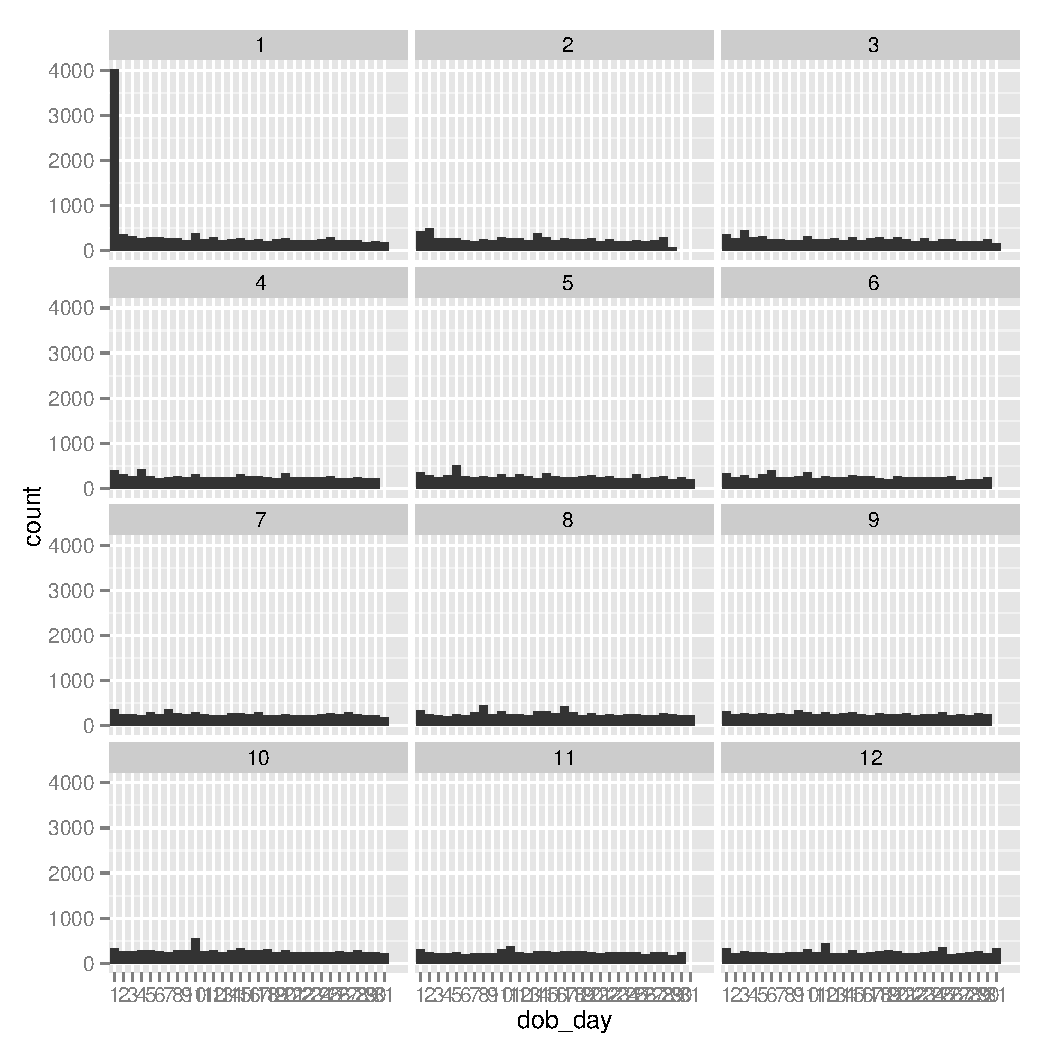
\includegraphics[]{/Users/RickyLim/Documents/OnlineLearning/DataAnalysisR/Codes/Lesson3/figs/user_bod.pdf}
\end{figure}

\begin{knitrout}
\definecolor{shadecolor}{rgb}{0.969, 0.969, 0.969}\color{fgcolor}\begin{kframe}
\begin{alltt}
\hlcom{# to resemble more normal distribution}
\hlkwd{summary}\hlstd{(}\hlkwd{log10}\hlstd{(pf}\hlopt{$}\hlstd{friend_count} \hlopt{+} \hlnum{1}\hlstd{))} \hlcom{# comparing in the order scale of 10}
\end{alltt}
\begin{verbatim}
##    Min. 1st Qu.  Median    Mean 3rd Qu.    Max. 
##   0.000   1.505   1.919   1.868   2.316   3.692
\end{verbatim}
\begin{alltt}
\hlkwd{summary}\hlstd{(}\hlkwd{sqrt}\hlstd{(pf}\hlopt{$}\hlstd{friend_count))}
\end{alltt}
\begin{verbatim}
##    Min. 1st Qu.  Median    Mean 3rd Qu.    Max. 
##   0.000   5.568   9.055  11.090  14.350  70.160
\end{verbatim}
\end{kframe}
\end{knitrout}

\begin{verbatim}
  Filename: lesson3.Rnw 
  Working directory: /Users/RickyLim/Documents/OnlineLearning/DataAnalysisR/Codes/Lesson3 
\end{verbatim}

\section{Metainfo}
\begin{knitrout}
\definecolor{shadecolor}{rgb}{0.969, 0.969, 0.969}\color{fgcolor}\begin{kframe}
\begin{alltt}
\hlkwd{sessionInfo}\hlstd{()}
\end{alltt}
\begin{verbatim}
## R version 3.1.1 (2014-07-10)
## Platform: x86_64-apple-darwin13.3.0 (64-bit)
## 
## locale:
## [1] en_US.UTF-8/en_US.UTF-8/en_US.UTF-8/C/en_US.UTF-8/en_US.UTF-8
## 
## attached base packages:
## [1] stats     graphics  grDevices utils     datasets  methods   base     
## 
## other attached packages:
## [1] ggplot2_1.0.0 knitr_1.7    
## 
## loaded via a namespace (and not attached):
##  [1] colorspace_1.2-4 digest_0.6.4     evaluate_0.5.5   formatR_1.0      grid_3.1.1      
##  [6] gtable_0.1.2     highr_0.3        labeling_0.3     MASS_7.3-33      munsell_0.4.2   
## [11] plyr_1.8.1       proto_0.3-10     Rcpp_0.11.2      reshape2_1.4     scales_0.2.4    
## [16] stringr_0.6.2    tcltk_3.1.1      tools_3.1.1
\end{verbatim}
\end{kframe}
\end{knitrout}



